\chapter{Methodology}
\label{cap:Methodology}

This chapter contains details about the followed methodology during the development stages of this project, a time planning for the development stages, the resulting
application of the methodology to this project, and the equipment (software and hardware) used during the development.

\section{Selected Methodology}\label{sec:DSDM}

The selected methodology for the development of this project has been based on the \acrfull{DSDM}, performing some minor adjustments so that the methodology ties in with the project's
needs.

This is an agile framework for software development. It was first published in 1995, with the aim of describing a methodology focused on quality, where the techniques 
for \acrfull{RAD} could be also applied in. The main feature of \acrshort{DSDM} is the use of prototyping techniques to guarantee the frequent delivery of software 
products to the end users\cite{dsdmintro}.

In terms of plannification, most methodologies select to establish a former definition of the desired functionalities to be developed, to then establish a latter time estimation
for the development of each functionality. \acrshort{DSDM}, on the other side, focuses more on establishing a time estimation for the development of the project, in which then the
amount of introduced functionality within the estimated time will be then organized\cite{agileplanning}.

\subsection{Principles of the selected methodology}\label{sec:DSDMPrinciples}

The \acrshort{DSDM} has eight basic principles on which it is sustained. These are:

\begin{enumerate}
    \item Focus on the business needs.
    \item Deliver the artifacts and products on time.
    \item Collaboration among team members.
    \item Build upon a strong basis.
    \item Iterative development.
    \item Continuous and clear communication among stakeholders.
    \item Control during the development of the project.
\end{enumerate}

\subsection{Techniques of the selected methodology}\label{sec:DSDMTechniques}

Throughout the course of the development of the project, \acrshort{DSDM} makes use of a wide-ranging set of techniques, that may be used either alone or in conjunction with
others according to the situation. The most important techniques (which are in fact used in some way in this project) are shown within \emph{figure \ref{fig:DSDMTechniques}},
and detailed within the following subsections.

\begin{figure}[H]
    \centering
    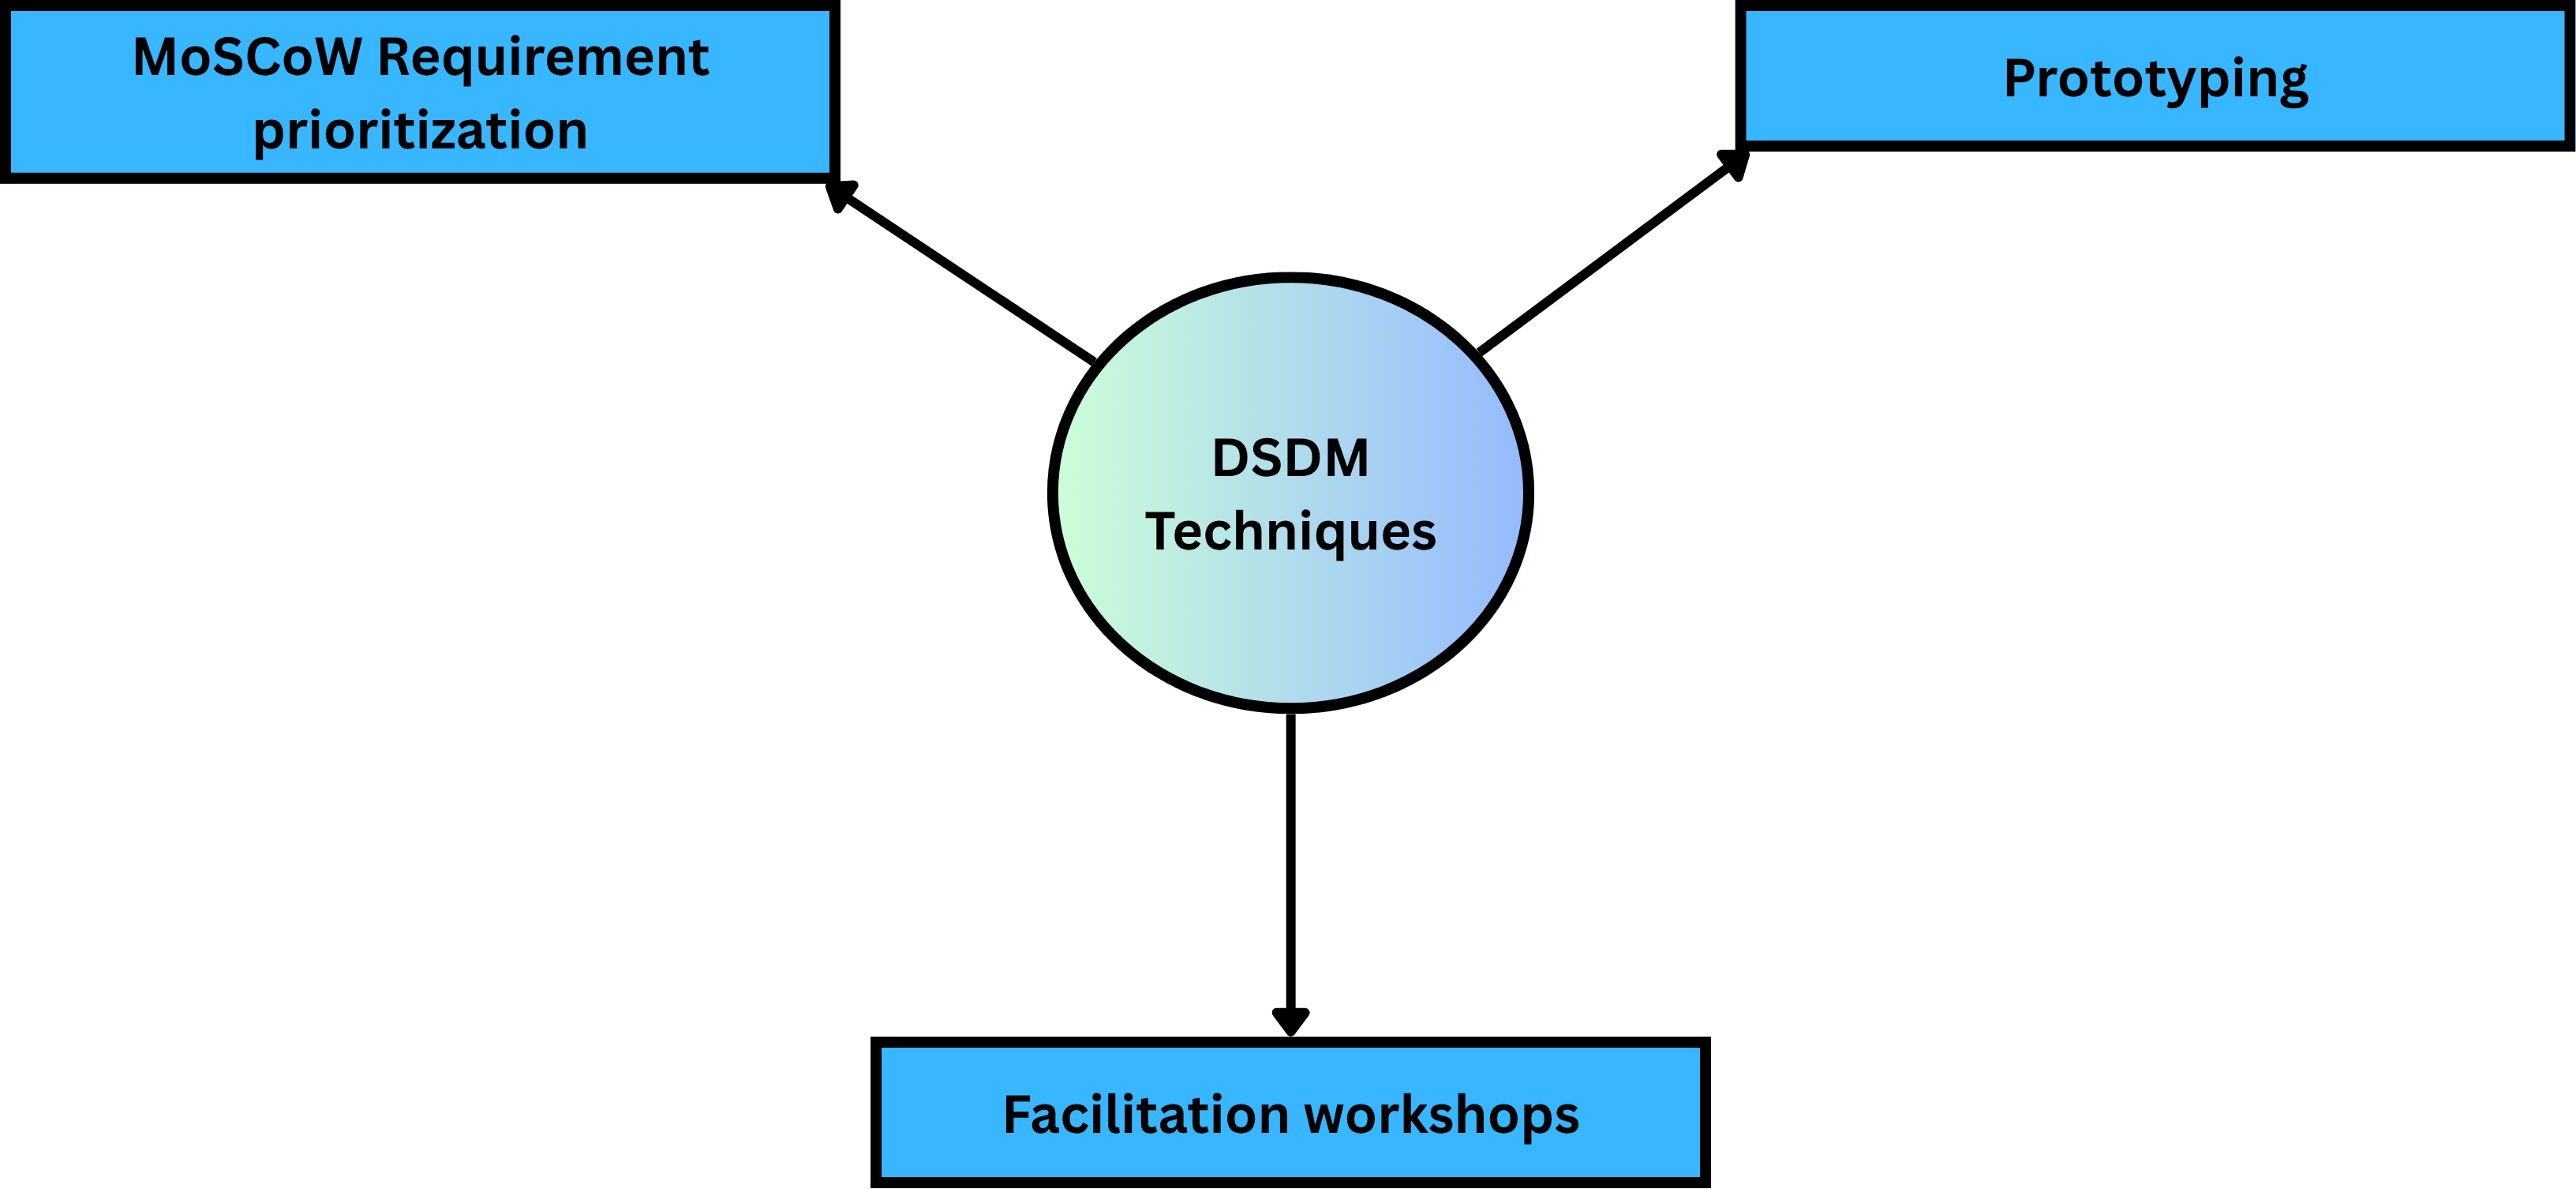
\includegraphics[width=0.8\linewidth]{figs/dsdm-techniques.png}
    \caption{Spider diagram containing techniques widely used in \acrshort{DSDM}.}
    \label{fig:DSDMTechniques}
\end{figure}


\subsubsection{MoSCoW requirement prioritization}\label{sec:MoSCoW}

The MoSCoW prioritization technique was created by software development consultant Dai Clegg in 1994, when teams at Oracle were using \acrshort{RAD} and needed a quick method to
establish requirement priorities. Some years later, in the 2000s, it became a popular technique specially in \acrshort{DSDM}\cite{moscow}.

Prioritization is an essential part of the planning phase of every project. It establishes which of the collected requirements will provide end users with the most value, and
should hence be worked on first. This prioritization is done classifying every single requirement under one of these categories: \emph{Must have}, \emph{Should have}, \emph{Could
have} and \emph{Won't have} (\emph{figure \ref{fig:MoSCoW}}). This classification gives all team members strategic knowledge about the impact of completing (or not) a requirement.

\begin{figure}[H]
    \centering
    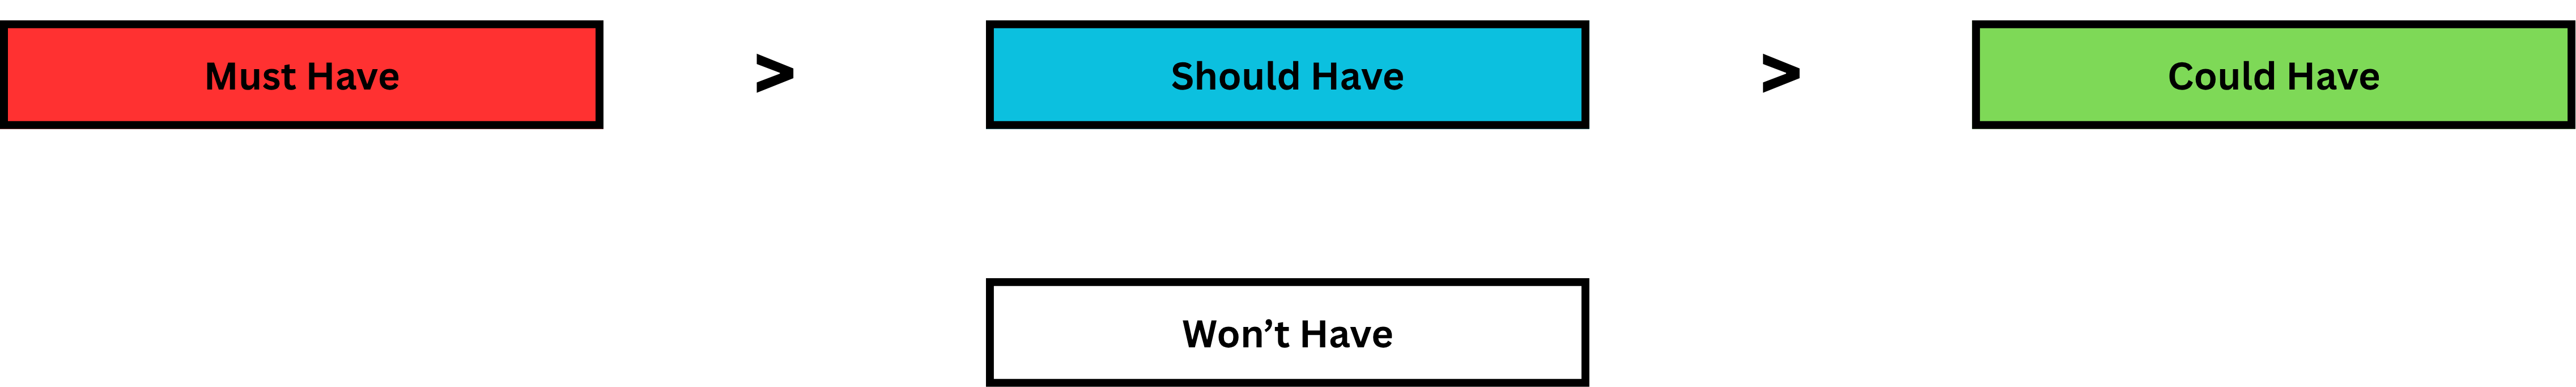
\includegraphics[width=0.8\linewidth]{figs/MosCow.png}
    \caption{MoSCoW prioritization establishes four different priority levels for a requirement.}
    \label{fig:MoSCoW}
\end{figure}

\begin{itemize}
    \item \textbf{Must have: }they are paramount to achieve the project's success. Requirements classified under this category will be the first ones to be completed, since
    they have the greatest importance.

    \item \textbf{Should have: }while they are not essential, they also hold great value for the project, so they should be developed whenever possible.
    
    \item \textbf{Could have: }these requirements are mostly an additive to the baseline of the project, which would increase the satisfaction level of the end users. They will
    only be developed once the baseline is completed, and there are enough time and resources to dedicate to them.

    \item \textbf{Won't have: }this category contains requirements that may hold any importance within the project, but because of limitations on time and resources,
    they will be discarded from the scope of this project's phase. These requirements could be set to be developed in the future phases.
\end{itemize}


\subsubsection{Prototyping}\label{sec:prototyping}

In order to have a shorter delivery interval, \acrshort{DSDM} uses evolutionary prototyping techniques for the development of user requirements.

The main aim of evolutionary prototyping is to carry out a software development production process in an iterative and incremental approach. This means that multiple iterations
of the software development lifecycle will be performed, each of them producing an increment of the system. Although the distinction between products and prototypes in this technique
is fuzzy, the result of the first iterations will be considered prototypes, since they are not near to the full functionality of the final target system\cite{prototyping}.

\subsubsection{Facilitation workshops}\label{sec:facilitationWorkshops}

These workshops are essentially meetings in which the stakeholders of the project meet with a specific objective related to the completion of deliverables. The purpose of the 
workshop is to reach clear solutions to the stated problems.

The development of these workshops is in many ways benneficial for the team:

\begin{itemize}
    \item The workshop is an ideal environment for brainstorming, as well as for discussion and developmen of the produced ideas.
    \item All the stakeholders get knowledge on the decisions made towards the project.
    \item Since all the stakeholders participate in the workshops, they will be able to propose ideas and take part in the decisive process.
    \item The decisions taken during the workshop are quick and precise.
\end{itemize}

\subsection{Project lifecycle in \acrshort{DSDM}}\label{sec:DSDMLifecycle}

The \acrshort{DSDM} methodology divides a project into seven phases to be completed sequentially. These phases are shown within \emph{figure \ref{fig:DSDMLifecycle}}.

\begin{figure}[H]
    \centering
    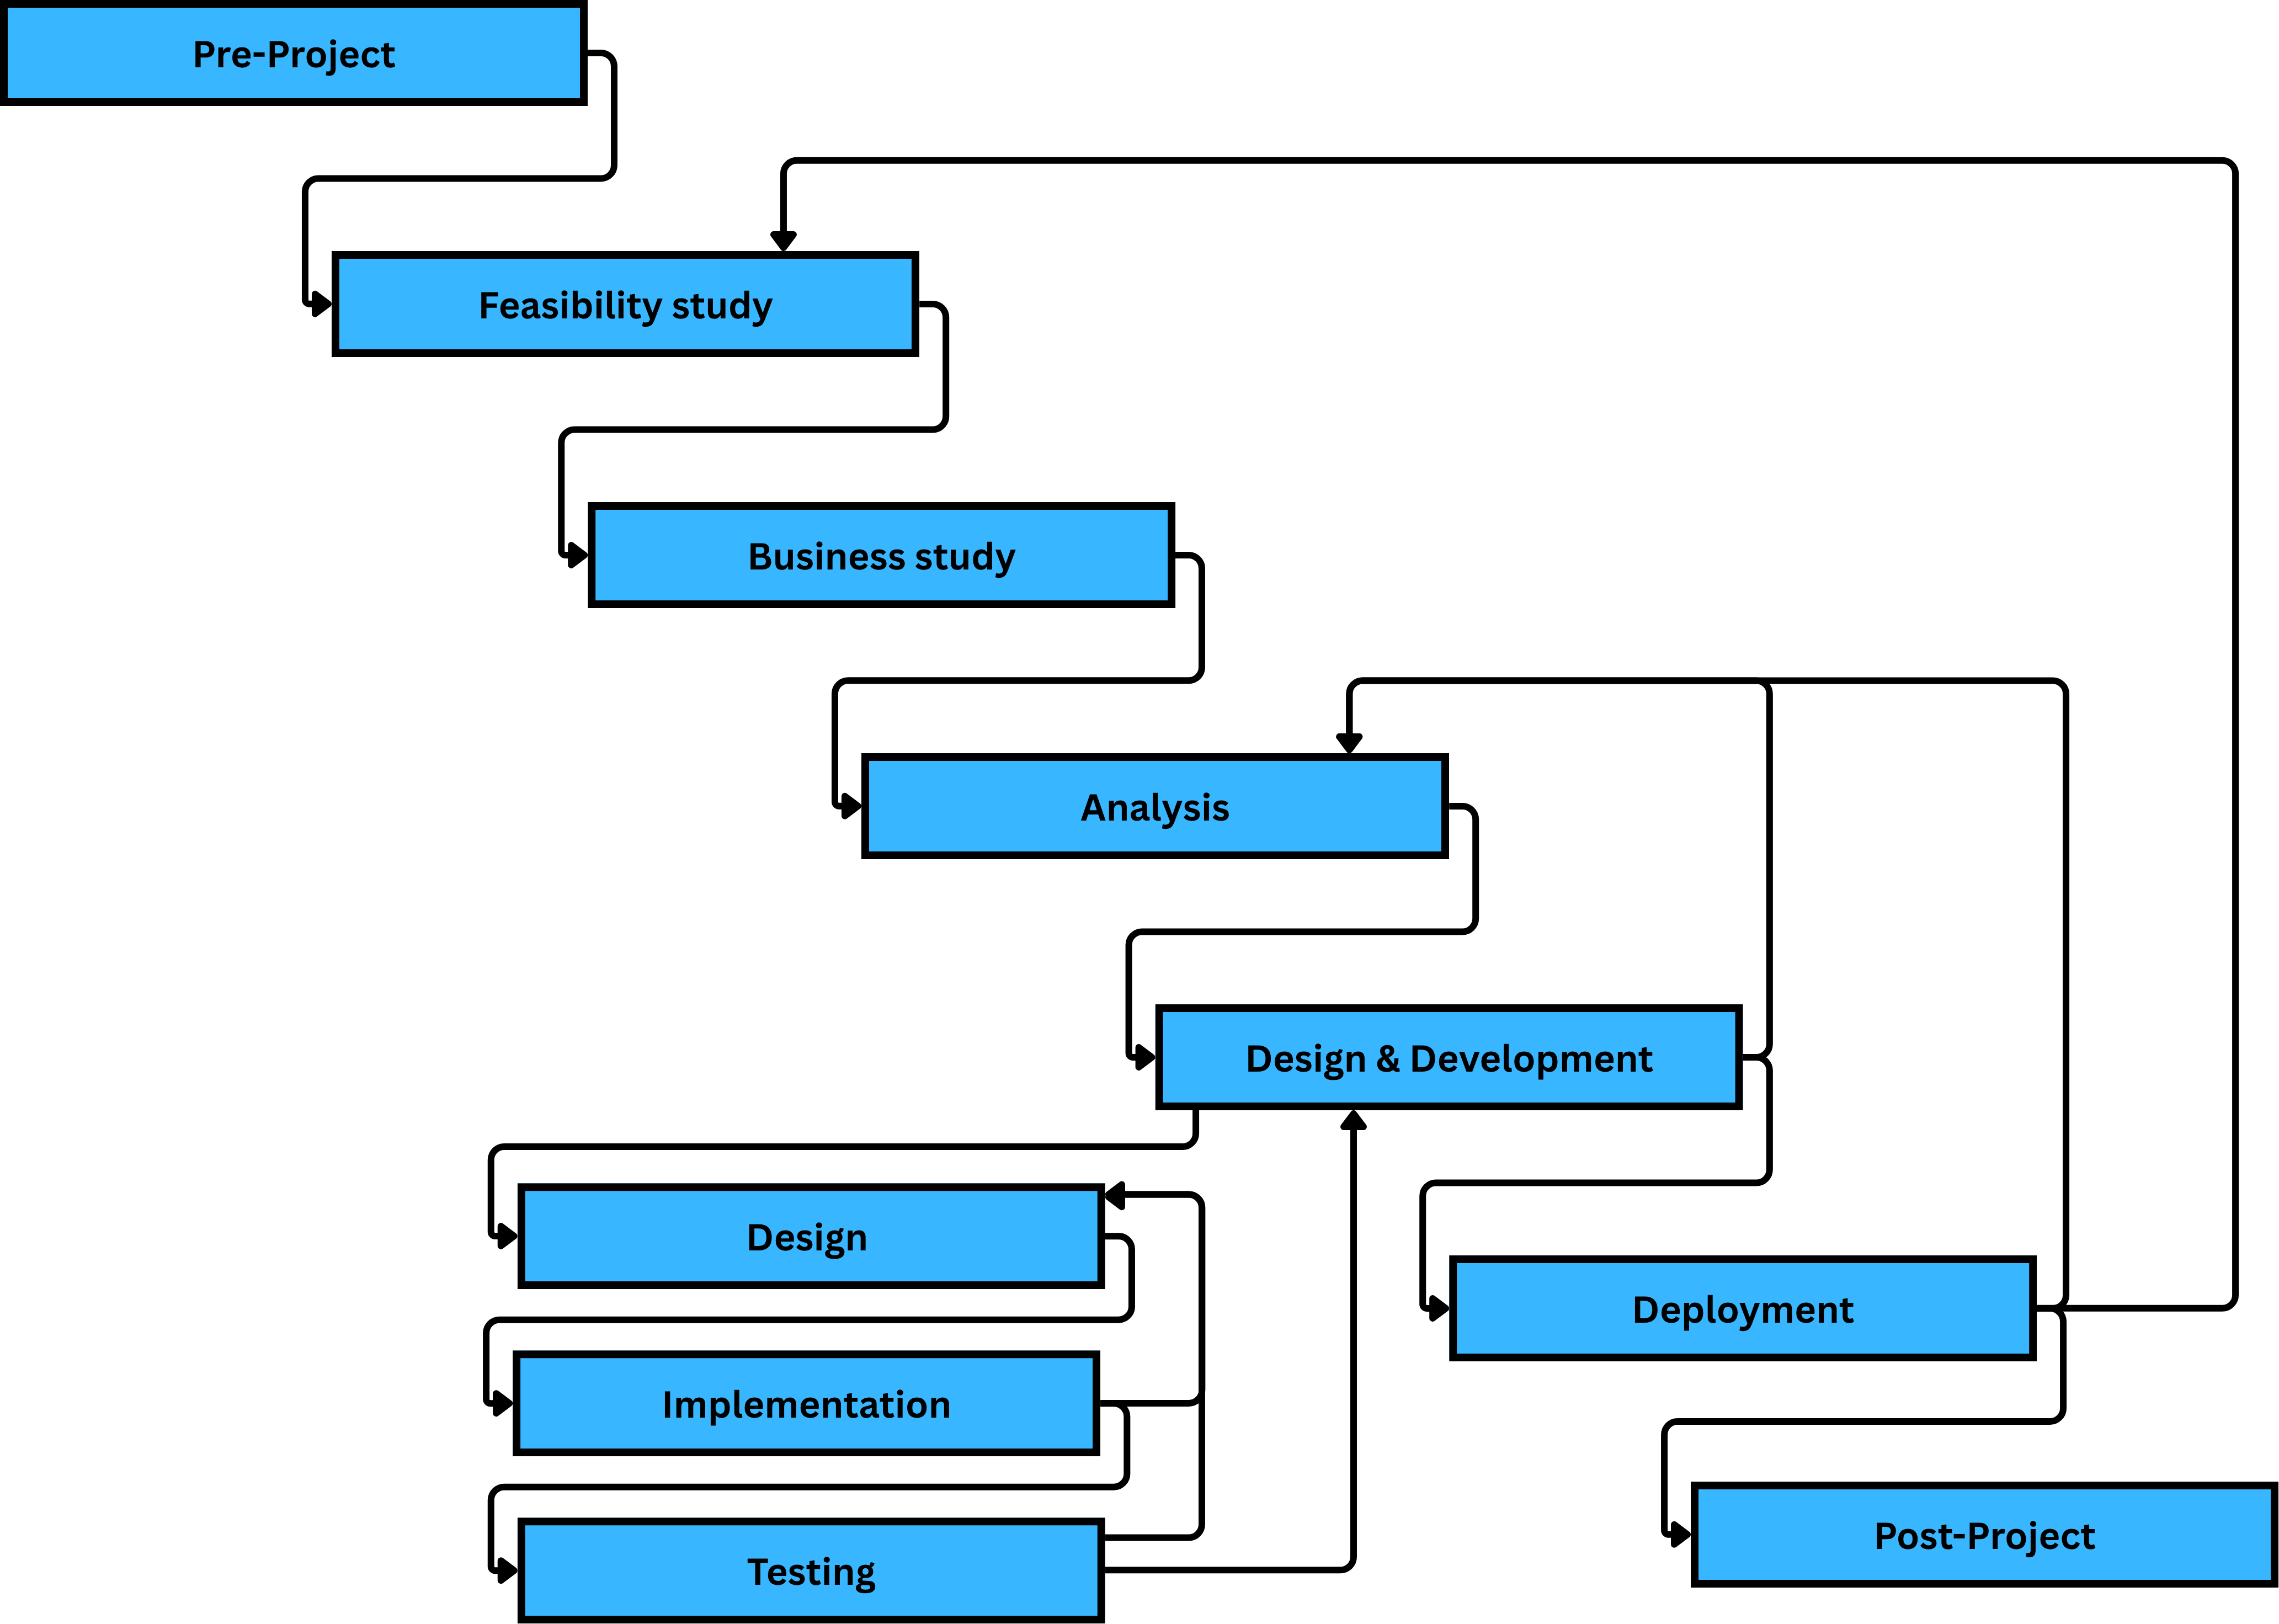
\includegraphics[width=0.8\linewidth]{figs/dsdm-lifecycle.png}
    \caption{The lifecycle of a project, according to \acrshort{DSDM}-based methodologies.}
    \label{fig:DSDMLifecycle}
\end{figure}

\begin{itemize}
    \item \textbf{Pre-project: }this phase has the aim of verifying the establishment of the project over a real need. As well as diagnosing the availability of resources to perform
    a feasibility study.

    \item  \textbf{Feasibility study: }apart from evaluating the adequacy of the use of \acrshort{DSDM} for the development of the project, the techniques to be employed are decided and the
    balance between opportunities and risks upon development is presented. The outputs of this phase include a feasibility report and a provisional project development plan.

    \item \textbf{Business study: }the main aspects of the domain is analyzed, as well as the pontential technologies to be used. The affected business processes are identified,
    along with the components of the target system and the architecture of the system. After this, an initial prototype (which can be far different from the final look of the target
    system) is then created.

    \item \textbf{Analysis: }The first phase of the iterative and incremental development loop. The outputs include a prioritized requirement list, the analysis report
    made on those same requirements, and a risk analysis.

    \item \textbf{Design and development: }the iterative phase where the system is properly built. The low-level component interfaces are designed, to then provide an implementation
    of the system. This phase iterates until obtaining a target system that complies with, at least, the minimal specification formed by the requirements previously agreed.

    \item \textbf{Deployment: }This is the phase englobing the process by which the developed system is integrated within the end user's infrastructure, and consequentially delivered
    to them. On integration, the end user(s) receive a user's manual with all the information needed to correctly make use of the system. Depending on how complex this integration is,
    it is possible to carry out this phase iteratively.

    \item \textbf{Post-project: }After the project ends, an evaluation is made based on whether the specified objectives were satisfactorily fulfilled, and a list of lessons learned is elaborated.
    If some requirements were not fulfilled within the specified time, they could be left for future work on another project.
\end{itemize}

\subsection{Roles in \acrshort{DSDM}}\label{sec:DSDMRoles}

The \acrshort{DSDM} methodology defines fifteen different roles for all the stakeholders of a project. Below, there is an explanation of the most important ones:

\begin{itemize}
    \item \textbf{Developer: }the role assigned to every member of the development team. That is, analysts, designers, programers and testers. These people directly participate
    in the creation of the system, specially within the \emph{Analysis} and \emph{Design and development} phases.
    
    \item \textbf{Technical coordinator: }assigned to those with the responsibility of guaranteeing the quality of the project and defining the architecture of the target
    system.
    
    \item \textbf{Visionary: }assigned to that team member that better understands the business objectives. They have the responsibility of ensuring the rapid completion of
    essential requirements (which according to the MosCow prioritization correspond to the ones labelled as \emph{Must Have}), as well as supervising that the project goes well.
    
    \item \textbf{Executive sponsor: }role assigned to the stakeholders belonging to the end users' organization, and holds the financial power and authority over the project. Stakeholders
    with this role hold great importance in decision-making.
\end{itemize}

\section{Application of the selected Methodology to the project}

This section takes the techniques, phases and roles enumerated and detailed in the previous section to then provide a summary of how and to what extent were they applied
to the project. On first place, the application of the aforementioned roles will be detailed, to then make a summary of the obtained requirements and their acquirement method,
their classification following the MosCoW technique, and how iterations will be classified according to the represented progress type. Finally, the tentative time estimation
per iteration will be presented, along with the actual duration of the iterations.

\subsection{Roles assignation}

According to the role definition made within \emph{section \ref{sec:DSDMRoles}}, the roles within the project have been distributed according to the principles defined in
\acrshort{DSDM}. The resulting assignation is the following:

\begin{itemize}
    \item \textbf{Developer: }the only person to which this role has been assigned is the author of this document, Miguel Ángel Ruiz Arreaza. He is responsible of compiling
    the project's requirements, as well as building the target system. He is considered as multidisciplinary, carrying out the responsibility of an analyst, a designer,
    a programmer and a tester.

    \item \textbf{Technical coordinator: }this role has been assigned to the tutor of this Final Degree Project. He will be in charge of coordinating
    the development and integration and to guarantee the technical quality within this project.

    \item \textbf{Visionary: }the co-tutor of this project has been assigned this role. He will be in charge of coordinating the development
    team with the executive sponsor, so as to assure the alignment and the development of this project with the business interests and objectives.

    \item \textbf{Executive sponsor: }the assignment of this role goes to the \acrshort{CTO} of the end users' company, which has the responsibility of providing the necessary
    resources to develop the project.
\end{itemize}

\subsection{Requirement collection}

The following subsections detail the methodology employed to obtain information about the current state of the configuration management procedures of the end users, as well of
their preferences, needs and working methodologies. Once this methodology is explained, the results obtained from applying it will be described.

\subsubsection{Requirement collection method}

This project has the purpose of creating a system designed to provide value to the target company, which is UBOTICA Technologies. Hence, it is important to consider the needs 
of the employees that work with both \acrshort{ML} and \acrshort{DL} models and datasets, and who have to deal with the difficulty of not keeping track of the state of these. 
For this purpose, a set of interviews were conducted from November 18\textsuperscript{th},2024, to November 25\textsuperscript{th},2024. The selected sample was a group consisting
of six employees working in \acrshort{AI} and \acrshort{CV} tasks close to production environments. Additionally, four of the interviewees also affirmed to carry out research tasks
in environments far from production.

\subsubsection{Requirement collection results}

After conducting the interviews and taking important notes, these are the most important points that should be taken into account for producing a requirement specification:

\begin{itemize}
    \item The end users work at \acrshort{CV}, so the predominating dataset type is the image dataset. The system must do well at managing, moving and changing these.

    \item There is not any official set of important metadata, that are always present within every model or project. The model and project's necessary metadata changes with
    the purpose of the project. This means that the system must be flexible on the amount of metadata to introduce for a certain \acrshort{AI} model or dataset.

    \item Hyperparameters take a particularly important role in model trainings for the end users, since they define important measures, like the length of the image bands and
    the number of colour channels. The system must consider a special form of classifying hyperparameters upon the training of a model.

    \item Upon having two versions of an \acrshort{AI} model, many interviewees selected their datasets along with their labelling distribution, their input hyperparameters, 
    the model architectures and the achieved metrics as the main points of differentiation. This means the system must consider these as the main points of the configuration
    of a model training.

    \item According to most interviewees, new versions of \acrshort{AI} models are stored within a cloud configuration management platform, and registered under a new release. On
    the other side, datasets are stored in a cloud storage platform, separated only by name and with no version tracking, meaning multiple versions of a dataset may coexist within
    the platform, each one occupying its own space. The target system must solve this issue so as to make the storage of datasets more efficient and scalable.

    \item Each time the pipeline of a model training completes successfully, some internal software component of the company automatically generates a PDF report with the main information
    of the training: metrics, performance and the differences with the base model. It would be interesting for the target system to enable the compilation of these reports when model
    trainings are performed. However, this is not true for all the pipelining software tools used within the target company, to the inclusion of this report should be optional.

    \item A particular subject admitted to formerly use the traditional method for storing the configuration of models and datasets, but many inconveniences made them take the decision
    to change to more specialized configuration management systems, such as DVC or WandB. These are technologies mentioned within Chapter 3, and the adoption of a system that integrates these
    will be easier for some workers.

    \item Whilst there are still subjects that denied having much issue when spotting a certain model, all of the interviewed workers assure that downloading datasets is troublesome, either
    due to the download mechanisms of the cloud storage, the location of a dataset within the local file system, the internal company's storage device or the cloud platform, or even by the
    long download time.

    \item Many individuals reported that a checkout system would make the search for a dataset quite more easy and time-efficient.

    \item Some individuals made special emphasis on their need to be able to represent the purpose of the model in some way.

    \item While there are mixed opinions on the inclusion of a parameter tweaking mechanism, the number of subjects declaring this feature out of the scope of the project outnumbers those who
    want it within the system.

    \item Individuals shown particular interest in the inclusion of an \emph{experiment tracking} mechanism within the system, specifically one that can sort the metrics obtained from
    trainings so that users could spot the best-performing model at a glance.
\end{itemize}

After compiling all these important points, a software requirement specification was redacted, being the resulting compilation the one shown in \emph{table \ref{tab:functionalRequirements}}.

\begin{table}[H]
	\centering
	\caption{List of functional requirements of the project (previous to organization and priorization).}
	\label{tab:functionalRequirements}
	\begin{tabular}{ | c | p{12cm} |}
		\hline
		\textbf{Requirement ID} & \textbf{Requirement Description} \\ \hline
		FR1     & The system MUST keep ordered track of dataset configurations. \\ \hline
		FR1.1   & The system MUST detect changes in the size (rows and columns) of datasets. \\ \hline
		FR1.2   & The system MUST keep track of the routes where models and datasets are stored \\ \hline
        FR2     & The system MUST handle the concept of experiments.\\ \hline
        FR2.1   & The system MUST identify an experiment by its identification string, or ID.\\ \hline
        FR2.2   & The system MUST provide a mechanism for creating experiments. \\ \hline
        FR2.3   & The system MUST not Accept an experiment creation request that has no experiment name.\\ \hline
        FR2.4   & The system MUST separate commits from different experiments. \\ \hline
        FR2.5   & The system MUST provide a mechanism for deleting experiments. \\ \hline
        FR2.6   & The system MUST provide a mechanism for switching between experiments.\\ \hline
        FR3     & The system MUST keep ordered track of machine learning model configurations.\\ \hline
        FR3.1   & The system MUST track which dataset was used to train the model.\\ \hline
        FR3.2   & The system MUST track which dataset was used to validate the model.\\ \hline
        FR3.3   & The system MUST track which dataset was used to test the model. \\ \hline
        FR3.4   & The system MUST track the code used for programming the model's training. \\ \hline
        FR3.5   & The system MUST track the configuration of the model's hyperparameters and random parameters used in the training of an AI model. \\ \hline
        FR3.6   & The system MUST track the metrics achieved by an AI model. \\ \hline
        FR3.7   & The system MUST provide users with a mechanism to mark an AI model as currently deployed. \\ \hline
        FR3.8   & The system MUST keep track of the additional parameters used by an AI model if it handles domain-specific data. This will be tested for the domain of Earth Observation (EO). \\ \hline
        FR4     & The system MUST provide a mechanism for evaluating an AI model's metrics' goodness.\\ \hline
        FR4.1   & The system MUST provide a mechanism for choosing policies to evaluate an AI model's metrics' goodness.\\ \hline
        FR4.2   & The system MUST provide a mechanism for identifying the experiment or model with the best values on the chosen metrics.\\ \hline
        FR4.3   & The system SHOULD order the model trainings made on an experiment by the goodness of the values on the chosen metrics.\\ \hline
        FR5     & The system MUST provide a mechanism for visualizing the performance report for a trained AI model (if any).\\ \hline
        FR6     & The system MUST provide a mechanism to visualize the training graph of a model (this is, the graph that describes the progress of the metrics of a model after each epoch).\\ \hline
        FR7     & The system MUST provide users with a mechanism to commit changes to the configuration of an item (both a dataset and an AI model). \\ \hline
	\end{tabular}
\end{table}

Additionally, a list of non-functional requirements was created, based on the needs of the company, these are listed under \emph{table \ref{tab:nonFunctionalRequirements}}.

\begin{table}[H]
	\centering
	\caption{List of non-functional requirements of the project.}
	\label{tab:nonFunctionalRequirements}
	\begin{tabular}{ | c | p{12cm} |}
		\hline
		\textbf{Requirement ID} & \textbf{Requirement Description} \\ \hline
        NFR1    & The system MUST be modular by design. \\ \hline
        NFR1.1  & The system MUST be extensible. \\ \hline
        NFR1.2  & The system MUST be reusable. \\ \hline
        NFR2    & The system MUST be maintainable. \\ \hline
        NFR3    & The system MUST be testable. \\ \hline
        NFR4    & The system SHOULD be power efficient. \\ \hline
        NFR5    & The system MUST be scalable. \\ \hline
        NFR6    & The system MUST maintain transactional integrity. \\ \hline
        NFR7    & The system MUST be fault tolerant. \\ \hline
        NFR8    & The system MUST be flexible. \\ \hline
        NFR9    & The system MUST follow best practices for security. \\ \hline
        NFR10   & The system MUST be usable. \\ \hline
        NFR11   & The system MUST outperform the traditional method for model tracking and downloading (<2h). \\ \hline
	\end{tabular}
\end{table}

\subsection{Requirement organisation and prioritization}\label{sec:requirementOrganisation}

Since this complex project aims to complete an extensive list of requirements, the development team along with the visionary and the technical coordinator decided in a 
facilitated workshop held at January 15\textsuperscript{th},2025, that these requirements shall be reorganized and rearranged by the final specific objective to be
completed. That means the project should be divided into milestones. After performing some analysis, three main milestones were defined for the project to succeed:

\begin{enumerate}
    \item \textbf{Milestone 1 (code \emph{D}):} Development of Dataset Configuration Management features completed.
    \item \textbf{Milestone 2 (code \emph{M}):} Development of Model Configuration Management features completed.
    \item \textbf{Milestone 3 (code \emph{G}):} Development of General Configuration Management features completed.
\end{enumerate}

Given these milestone definitions, the requirement specification was updated so that every functional requirement was classified into one of the milestones. The new 
rearranged requirements would be numbered and identified by the milestone they contribute to, resulting into the specifications shown in \emph{table \ref{tab:requirementsMilestone1}}, \emph{table \ref{tab:requirementsMilestone2}} and \emph{table \ref{tab:requirementsMilestone3}}.

Additionally, these tables incorporate the priorities following the procedures described in \emph{section \ref{sec:MoSCoW}}.

\begin{table}[H]
	\centering
	\caption{List of functional requirements belonging to milestone 1.}
	\label{tab:requirementsMilestone1}
	\begin{tabular}{ | c | p{9cm} | p{3cm} |}
		\hline
		\textbf{Requirement ID} & \textbf{Requirement Description} & \textbf{priority (MoSCoW)} \\ \hline
		DFR1     & The system MUST keep ordered track of dataset configurations.                    & Must have\\ \hline
		DFR1.1   & The system MUST detect changes in the size (rows and columns) of datasets.       & Must have\\ \hline
		DFR1.2   & The system MUST keep track of the routes where models and datasets are stored    & Must have\\ \hline
	\end{tabular}
\end{table}

\begin{longtable}{| c | p{9cm} | p{3cm} |} % La alineación de la tabla ya se define aquí.
    \caption{List of functional requirements belonging to milestone 2.}\\ % Captura para la tabla
    \toprule
    \label{tab:requirementsMilestone2}\\ 
    \textbf{Requirement ID} & \textbf{Requirement Description} & \textbf{priority (MoSCoW)} \\
    \endfirsthead % <-- Cierre del encabezado de la primera página

    % Este es el encabezado que se repite en cada página subsiguiente
    \multicolumn{3}{c}%
    {{\bfseries \tablename\ \thetable{}}} \\ \hline
    \textbf{Requirement ID} & \textbf{Requirement Description} & \textbf{priority (MoSCoW)} \\
    \endhead % <-- Cierre del encabezado para el resto de páginas

    \multicolumn{3}{r}{\textit{Continuing on the next page}} \\
    \endfoot % <-- Pie de tabla para todas las páginas excepto la última

    \endlastfoot % <-- Pie de tabla para la última página

    % Contenido de tu tabla
    \hline
    MFR1     & The system MUST handle the concept of experiments. & Must have \\ \hline
    MFR1.1   & The system MUST identify an experiment by its identification string, or ID. & Must have \\ \hline
    MFR1.2   & The system MUST provide a mechanism for creating experiments. & Must have \\ \hline
    MFR1.3   & The system MUST not accept an experiment creation request that has no experiment name. & Must have \\ \hline
    MFR1.4   & The system MUST separate commits from different experiments. & Must have \\ \hline
    MFR1.5   & The system MUST provide a mechanism for deleting experiments. & Must have \\ \hline
    MFR1.6   & The system MUST provide a mechanism for switching between experiments. & Must have \\ \hline
    MFR2     & The system MUST keep ordered track of machine learning model configurations. & Must have \\ \hline
    MFR2.1   & The system MUST track which dataset was used to train the model. & Must have \\ \hline
    MFR2.2   & The system MUST track which dataset was used to validate the model. & Must have \\ \hline
    MFR2.3   & The system MUST track which dataset was used to test the model. & Must have \\ \hline
    MFR2.4   & The system MUST track the code used for programming the model's training. & Must have \\ \hline
    MFR2.5   & The system MUST track the configuration of the model's hyperparameters and random parameters used in the training of an AI model. & Must have \\ \hline
    MFR2.6   & The system MUST track the metrics achieved by an AI model. & Must have \\ \hline
    MFR2.7   & The system MUST provide users with a mechanism to mark an AI model as currently deployed. & Should have \\ \hline
    MFR2.8   & The system MUST keep track of the additional parameters used by an AI model if it handles domain-specific data. This will be tested for the domain of Earth Observation. & Must have \\ \hline
    MFR3     & The system MUST provide a mechanism for evaluating an AI model's metrics' goodness. & Should have \\ \hline
    MFR3.1   & The system MUST provide a mechanism for choosing policies to evaluate an AI model's metrics' goodness. & Should have \\ \hline
    MFR3.2   & The system MUST provide a mechanism for identifying the experiment or model with the best values on the chosen metrics. & Should have \\ \hline
    MFR3.3   & The system SHOULD order the model trainings made on an experiment by the goodness of the values on the chosen metrics. & Should have \\ \hline
    MFR4     & The system MUST provide a mechanism for visualizing the performance report for a trained AI model (if any). & Should have \\ \hline
    MFR5     & The system MUST provide a mechanism to visualize the training graph of a model (this is, the graph that describes the progress of the metrics of a model after each epoch). & Could have \\ \hline
\end{longtable}


\begin{table}[H]
	\centering
	\caption{List of functional requirements belonging to milestone 3 (expanded due to space availability).}
	\label{tab:requirementsMilestone3}
	\begin{tabular}{ | c | p{9cm} | p{3cm} |}
		\hline
		\textbf{Requirement ID} & \textbf{Requirement Description} & \textbf{priority (MoSCoW)} \\ \hline
        GFR1     & The system MUST provide users with a mechanism to commit changes to the configuration of an item (both a dataset and an AI model).   & Must have \\ \hline
        GFR1.1   & The system MUST Identify commits by their Identification string, or ID.   & Must have \\ \hline
        GFR1.2   & The system MUST provide a mechanism for creating commits.   & Must have \\ \hline
        GFR1.3   & The system MUST not Accept the creation of a commit that does not have a commit title.    & Must have\\ \hline
        GFR1.4   & The system MUST allow users to leave a commit message when building up a commit.    & Must have\\ \hline
        GFR1.5   & The system MUST provide users with a mechanism to push a commit to a certain remote repository location.    & Must have\\ \hline
        GFR1.6   & The system MUST provide users with a mechanism to go back to a previous commit.    & Must have\\ \hline
        GFR1.7   & The system MUST be able to handle two instances of a same dataset or model, in different versions, within the same repository.    & Must have\\ \hline
	\end{tabular}
\end{table}

\subsection{Iteration planning}

According to \emph{section \ref{sec:DSDMTechniques}}, prototyping is one of the main techniques within \acrshort{DSDM}-based methodologies. Hence, the iterations of the development
of the project have been organised according to prototype production. In other words, the output of an iteration of the \emph{Design and development} phase of the project is a project
prototype.

Each prototype will be assigned a subset of requirements of a specific milestone, following the milestone definition made at \emph{section \ref{sec:requirementOrganisation}}. The prototype
(and therefore, the iteration of the project) is considered as completed when all the requirements of the prototype are developed. The development of a prototype may require performing minor
changes on the development of previous prototypes. This fact motivates the definition of a versioning protocol for these prototypes, which will be defined in the following subsection. Right
afterwards, the prototypes will be defined and then arranged into the roadmap of the project.

\subsubsection{Prototype version control protocol}

Given the three milestones defined at \emph{section \ref{sec:requirementOrganisation}}, the name of a prototype will consist of the code of the milestone it corresponds to, 
and the iteration number it corresponds to within that same milestone (e.g., the first prototype for Milestone 3 would be called \emph{G1}).

For any addition to an already-developed prototype related with the requirements contained within it (e.g., a hotfix), semantic versioning will be used.
For instance, if a hotfix is needed to prototype \emph{G1}, the new version of the prototype will be called \emph{G1.0.1}. For minor versions, the second number will be increased. Of 
course, a higher major number for a prototype will indicate that it includes the past prototypes for its milestone\cite{semanticversioning}. If no prototypes have been developed
for a particular milestone at a given moment, the iteration number for that milestone will be considered 0.

The name for a version of the system will be the mixture of all the prototypes present up to the point the version is released. As an example, a version of the system that 
only contains the first prototypes of milestones 1 and 2 would be called \emph{D1M1G0}.

\subsubsection{List of prototypes of the project}

\paragraph{Prototypes for milestone 1}

\begin{itemize}
    \item \textbf{Prototype D1: }Provides the necessary mechanisms for the system to be able to integrate and transparently locate a dataset in the system (establishing a versioning protocol).

    \item \textbf{Prototype D2: }Apart from locating a dataset, the system is able to detect simple changes in the datasets, particularly in the number and content of the features and instances
    contained within them. Additionally, the system will be able to bring a dataset from a specific location to the user.
\end{itemize}

\paragraph{Prototypes for milestone 2}

\begin{itemize}
    \item \textbf{Prototype M1: }this inital prototype is focused on the integration of the concept of \emph{experiments} in the system, being able to create and track multiple 
    experiments, apart from sepparating the progress made among the different experiments.
    \item \textbf{Prototype M2: }once the system is able to differenciate the different experiments, the system must be able to track the different characteristics of a model
    upon training. This involves tracking the used datasets, the hyperparameters used, the metrics achieved, and experiment data related to the domain of application (in the 
    current case, the domain of Earth Observation).
    \item \textbf{Prototype M3: }the system is able to used the historically collected metrics from an experiment in order to extract key information like, for example, which
    of the historically performed experiment runs provided the best performance. Additionally, it provides mechanisms for visualizing both the performance report and the 
    training graph produced by the training of an \acrshort{AI} model.
\end{itemize}


\paragraph{Prototypes for milestone 3}

\begin{itemize}
    \item \textbf{Prototype G1: }The system provides a mechanism for users to commit changes to an item (a dataset or an AI model) in order to store them as historical versions in the system.
\end{itemize}

\subsubsection{Roadmap of the project}

On \emph{figure \ref{fig:roadmap}}, the dependencies among iterations (and hence, the dependencies among the prototypes) are shown. The main dependencies encountered are:

\begin{enumerate}
    \item Prototypes \emph{D2} and \emph{M2} depend both on \emph{G1}, since both of these prototypes generate items that may be of great value to commit. Hence, it would be valuable 
    to already have mechanisms that allow to store the items within a configuration management system. This makes \emph{G1} the prototype on which more iterations depend and, therefore,
    motivates it to be the first one to be completed.

    \item Prototype \emph{M2} depends on prototype \emph{D1}, since the former needs to identify the datasets used upon the training process of a model, and will use whatever versioning
    system is defined at the latter to reference these datasets.
\end{enumerate}

Considering the purpose of the prototypes and their dependencies, the designed roadmap is shown at \emph{table \ref{tab:roadmap}}.

\begin{table}[H]
	\centering
	\caption{Roadmap for the project. For details about the stages and dependencies, see \emph{figure \ref{fig:roadmap}}.}
	\label{tab:roadmap}
	\begin{tabular}{ | c | p{9cm} |}
		\hline
		\textbf{Iteration} & \textbf{Prototypes and Phases involved} \\ \hline
        Iteration 1  & \begin{itemize} \item Milestone 3 Analysis \item Prototype \emph{G1} \end{itemize} \\ \hline
        Iteration 2  & \begin{itemize} \item Milestone 1 Analysis \item Prototype \emph{D1} \end{itemize} \\ \hline
        Iteration 3  & \begin{itemize} \item Prototype \emph{D2} \end{itemize} \\ \hline
        Iteration 4  & \begin{itemize} \item Milestone 2 Analysis \item Prototype \emph{M1} \end{itemize} \\ \hline
        Iteration 5  & \begin{itemize} \item Prototype \emph{M2} \end{itemize} \\ \hline
        Iteration 6  & \begin{itemize} \item Prototype \emph{M3} \end{itemize} \\ \hline
	\end{tabular}
\end{table}


\subsection{Time estimations for the project}

With the clear picture of what prototypes provide more value and have more dependencies, an estimation was made of the 
investment of the time that will be required to carry out each iteration of the project.


\subsubsection{Early time estimation}

A first estimation was made before the beginning of the \emph{Analysis} phase of the project, and can be seen in \emph{table \ref{tab:firstTimeEstimation}}. 
The protototypes are ordered sequentially according to the proposed development order, prioritizing those iterations whose output
prototype constitutes a dependency to others. The higher the number of development order, the further in the timeline the 
iteration shall be scheduled.

\begin{table}[H]
	\centering
	\caption{Time estimations for all the project iterations.}
	\label{tab:firstTimeEstimation}
	\begin{tabular}{ | c | c |}
		\hline
		\textbf{Iteration} & \textbf{Time estimation (Days)} \\ \hline
        Iteration 1     & 15 \\ \hline
        Iteration 2     & 15 \\ \hline
        Iteration 3     & 10 \\ \hline
        Iteration 4     & 15 \\ \hline
        Iteration 5     & 10 \\ \hline
        Iteration 6     & 10 \\ \hline
        \textbf{Total}  & 75 \\ \hline
	\end{tabular}
\end{table}


\subsubsection{Actual time duration}

During the course of the project, the time spent in each iteration differed from the initial time estimation. The actual 
time durations are shown in \emph{table \ref{tab:actualTimeDurations}}.

\begin{table}[H]
    \centering
    \caption{Actual time durations for all the project iterations.}
    \label{tab:actualTimeDurations}
    \begin{tabular}{ | c | c |}
        \hline
        \textbf{Iteration} & \textbf{Time duration (Days)} \\ \hline
        Iteration 1     & 18 \\ \hline
        Iteration 2     & 21 \\ \hline
        Iteration 3     & 9 \\ \hline
        Iteration 4     & 20 \\ \hline
        Iteration 5     & 14 \\ \hline
        Iteration 6     & 9  \\ \hline
        \textbf{Total}  & 91  \\ \hline
    \end{tabular}
\end{table}

The main reason for this 16-day difference is mainly because of prototypes \emph{D1} and \emph{M1}, which required more time to be completed in order for the development
team to be familiarized themselves with the used technological tools used, and finding the ways for them to be integrated within the project. The fact that an initial analysis was also 
included within iterations 2 and 4 is another reason for this difference.

\section{Employed equipment and resources}

A key aspect of the description of the project is not only the techniques used to carry out the development, but also the resources (in this case, hardware and software)
utilized in the process. Coming on this section and its subsections, the details about the different equipment and resources used within the development of MADTrack.

\subsection{Hardware resources}

Hardware resources constitute the set of physical devices and peripherals used to carry out the development of the project.

\subsubsection{Computer}

During the development of the project, the target company provided the development team with a laptop computer. This computer is the main means through which the main programming
were performed, through which the main documentation and this document were written. This laptop was also used during the different facilitation workshops held during the course
of the project.

This computer model is HP OMEN 16-b0xxx, running on the specifications shown at \emph{table \ref{tab:computerSpecs}}.

\begin{table}[H]
    \centering
    \caption{Specifications of the computer used in the development of the project.}
    \label{tab:computerSpecs}
    \begin{tabular}{ | r | l |}
        \hline
        \textbf{Operating System} & Ubuntu 24.04 LTS \\ \hline
        \textbf{CPU} & Intel Core i5-1035G1 2.00 GHz \\ \hline
        \textbf{CPU Cores} & 16 \\ \hline
        \textbf{External GPU} & NVIDIA GeForce RTX™ 3060 Laptop GPU \\ \hline
        \textbf{Integrated GPU} & Intel® UHD Graphics (TGL GT1) \\ \hline
        \textbf{RAM Memory} & Tiger Lake-H 16GB (2x8GB) \\ \hline
        \textbf{Storage Memory} & 1TB NVME™ SSD M.2 \\ \hline
    \end{tabular}
\end{table}

\subsection{Software resources}

Software is the intangible material and tools within computers, in this case those that are used to develop the project.

\subsubsection{Programming Languages}

The programming languages used for implementing the components of the project have been:

\begin{itemize}
    \item \textbf{Python: }It is the programming language with the most synergies with \acrshort{AI} models and libraries, incorporating powerful frameworks like
    SKLearn, Pytorch or Tensorflow. It also provides simple yet effective libraries and utilities to carry out client-server communications.
    \item \textbf{Makefile: }the programming language used for automatizing tasks like compilation, execution and environment cleaning, offering a simple, flexible
    and effective tool for the deployment and testing of the project.
    \item \textbf{Bash Scripting: }used for the automatic deployment of the Tracking Server, a component that will be described in more detail within the coming chapters.
\end{itemize}

\subsubsection{Specialized software and libraries}

Specialized software and libraries enable developers to perform certain particular complex tasks without reinventing software. These are the libraries and specialized software
used during the course of the development of the project:

\begin{itemize}
    \item \textbf{\emph{GitPython}: }a Python library that handles operations on Git repositories. It will be used for generating commits in local repositories and initializing them,
    as well as accessing other Git operations.

    \item \textbf{\emph{DVC}: }an open-source software that is also a Python library that provides mechanisms for handling operations using the DVC tool. DVC is a tool that enables configuration management 
    for big datasets inside a Git repository.

    \item \textbf{\emph{MLFlow}: }an open-source software that is also a Python library. Provides a REST API for tracking and logging machine learning experiments.

    \item \textbf{\emph{Docker}: }a software dedicated to managing containers, which are isolated environments for running applications. It is used for the creation of containers as part
    of the deployment of the Tracking Server.

    \item \textbf{\emph{Pandas}: }a Python library that provides high-performance, easy-to-use data structures and data analysis tools for the Python programming language. It is used for retrieving certain fields
    out of a training configuration.

    \item \textbf{\emph{PyTest}: }a Python library that provides a simple and flexible testing framework. It was used for preparing, running and validating the different unit tests of the components of the project.
\end{itemize}

\subsubsection{\acrfull{IDE}}

The only \acrshort{IDE} used during the development of the project is \emph{Visual Studio Code}, which is a free and open-source code editor that provides a rich set of utilities
for software developers, such as a file navigator, a wide-ranging variety of extensions, and interactive language support for a wide range of programming languages.

\subsubsection{Versioning control}

The versioning control for this project was managed using \emph{Git} and its web storage service, \emph{GitHub}. It is the most used version control tool used for an immense variety of
software projects. Taking advantage of the use of these tools and platforms by the end users, it was decided to store this project's code within their environment, as well as make use of
it for keeping track of the development state of the project. 

As an additional fact, the use of the \emph{fork} mechanism provided by GitHub was particularly useful for developing an integration
test between the target system and a generic version of the pipeline used in real projects. Another functionality of GitHub that was vital for the correct versioning of the project was the
\emph{release} utility, which allows to create releases for the project and its components.

\subsubsection{Documentation tools}

The documentation of the project (as well as the documentation of the memory of this Final Degree Project) was developed using the following tools:

\begin{itemize}
    \item \textbf{\LaTeX: }this programming language is specialized on producing professional documents, such as papers or scientific reports. It is the main tool used
    for the production of this document.

    \item \textbf{Canva: }a web-based design tool that enables the creation of high-quality infographics. This was used for the creation of most of the project's non-UML
    diagrams (e.g., the dependency diagram of the stages of the project (\emph{figure \ref{fig:roadmap}})).

    \item \textbf{Visual Paradigm Online: }another web-based design tool specialized in UML diagrams. It was used specially for the creation of the project's use case diagrams.

    \item \textbf{Drawio: }another web-based design tool specialized in UML diagrams. It was used specially for the creation of the project's components' class diagrams.
\end{itemize}